\documentclass[10pt]{beamer}
\usetheme[
%%% options passed to the outer theme
%    progressstyle=movCircCnt,   %either fixedCircCnt, movCircCnt, or corner
%    rotationcw,          % change the rotation direction from counter-clockwise to clockwise
%    shownavsym          % show the navigation symbols
  ]{AAUsimple}
  
% If you want to change the colors of the various elements in the theme, edit and uncomment the following lines
% Change the bar and sidebar colors:
%\setbeamercolor{AAUsimple}{fg=red!20,bg=red}
%\setbeamercolor{sidebar}{bg=red!20}
% Change the color of the structural elements:
%\setbeamercolor{structure}{fg=red}
% Change the frame title text color:
%\setbeamercolor{frametitle}{fg=blue}
% Change the normal text color background:
%\setbeamercolor{normal text}{fg=black,bg=gray!10}
% ... and you can of course change a lot more - see the beamer user manual.

\usepackage[utf8]{inputenc}
\usepackage[english]{babel}
\usepackage[T1]{fontenc}
% Or whatever. Note that the encoding and the font should match. If T1
% does not look nice, try deleting the line with the fontenc.
\usepackage{helvet}

% colored hyperlinks
\newcommand{\chref}[2]{%
  \href{#1}{{\usebeamercolor[bg]{AAUsimple}#2}}%
}

\title{Context-Aware Home Automation Using Gestures on a Wearable}

\subtitle{}  % could also be a conference name

\date{June 22, 2016}

\author{
  Kasper Lind Sørensen,\\
  Simon Binderup Støvring
}

% - Give the names in the same order as they appear in the paper.
% - Use the \inst{?} command only if the authors have different
%   affiliation. See the beamer manual for an example

\institute[
%  {\includegraphics[scale=0.2]{aau_segl}}\\ %insert a company, department or university logo
  Aalborg University\\
  Denmark
] % optional - is placed in the bottom of the sidebar on every slide
{% is placed on the bottom of the title page
  Aalborg University\\
  Denmark
  
  %there must be an empty line above this line - otherwise some unwanted space is added between the university and the country (I do not know why;( )
}

% specify a logo on the titlepage (you can specify additional logos an include them in 
% institute command below
\pgfdeclareimage[height=1.5cm]{titlepagelogo}{AAUgraphics/aau_logo_new} % placed on the title page
%\pgfdeclareimage[height=1.5cm]{titlepagelogo2}{AAUgraphics/aau_logo_new} % placed on the title page
\titlegraphic{% is placed on the bottom of the title page
  \pgfuseimage{titlepagelogo}
%  \hspace{1cm}\pgfuseimage{titlepagelogo2}
}

\begin{document}
% the titlepage
{\aauwavesbg%
\begin{frame}[plain,noframenumbering] % the plain option removes the header from the title page
  \titlepage
\end{frame}}
%%%%%%%%%%%%%%%%

% % TOC
% \begin{frame}{Agenda}{}
% \tableofcontents
% \end{frame}
% %%%%%%%%%%%%%%%%

\chapter{Introduction}
\label{chap:introduction}

\section{Initial Problem}
\label{sec:initproblem}

In a previous report we documented the work on a system that integrated wearables into a home automation environment in order to provide an interface for controlling devices that are connected to the Internet \cite{prespecialisation}. This report is based on the work done in our previous report.

In the previous report \cite[pp. 1-4]{prespecialisation} we presented \cref{fig:wearables-trend,fig:smarthomestrend}. The figures show an increasing trend in wearables and smart homes. Common for wearables and smart homes are that they are both involved in the concept of Internet of Things. As both concepts are predicted to be an increasing trend, it is interesting to combine the two in order to make a system that provides an interface for controlling a smart home using a wearable device.

\begin{figure}[!hbt]
  \centering
  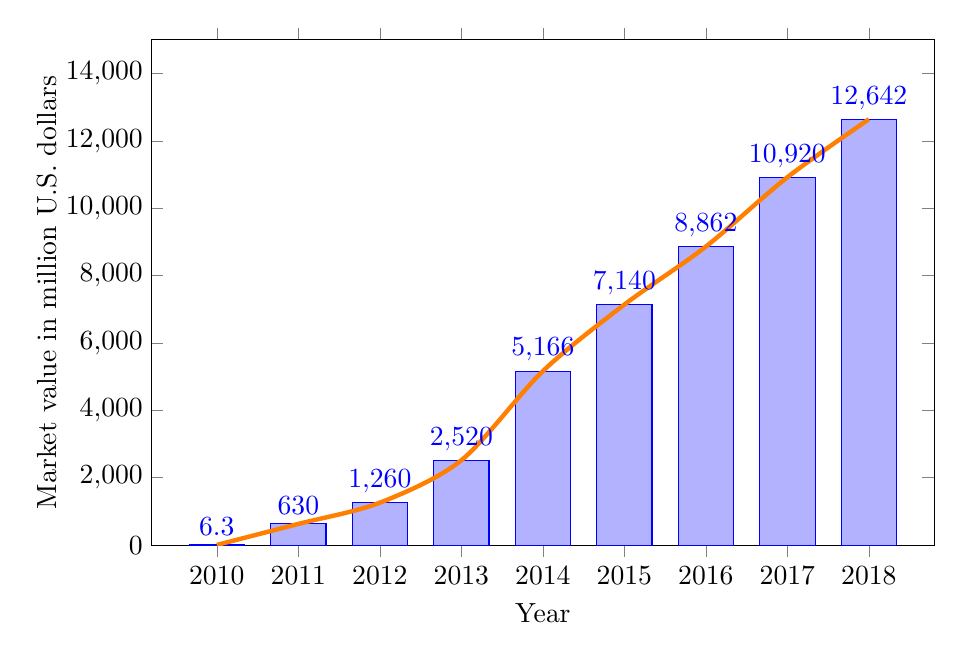
\begin{tikzpicture}
    \begin{axis}[
        height=8cm,
        width=0.95\textwidth,
        xlabel={Year},
        ylabel={Market value in million U.S. dollars},
        yticklabel style={align=right,inner sep=0pt,xshift=-0.3em},
        scaled y ticks = false,
        nodes near coords align={vertical},
        nodes near coords,
        xtick=data,
        symbolic x coords={2010, 2011, 2012, 2013, 2014, 2015, 2016, 2017, 2018},
        ymax=15000,
        ymin=0,
        ybar, 
        bar width=20pt
        ]
        \addplot coordinates {(2010, 6.3) (2011, 630) (2012, 1260) (2013, 2520) (2014, 5166) (2015, 7140) (2016, 8862) (2017, 10920) (2018, 12642)};
        \addplot [ultra thick,orange,line join=round,smooth, nodes near coords = ] coordinates {(2010, 6.3) (2011, 630) (2012, 1260) (2013, 2520) (2014, 5166) (2015, 7140) (2016, 8862) (2017, 10920) (2018, 12642)};
%        
    \end{axis}
\end{tikzpicture}
  \caption{Wearables trend based on sales and statistics. Data from \protect\cite{WEARABLESTRENDNUMBERS}.}
  \label{fig:wearables-trend}
\end{figure}

\begin{figure}[!hbt]
  \centering
  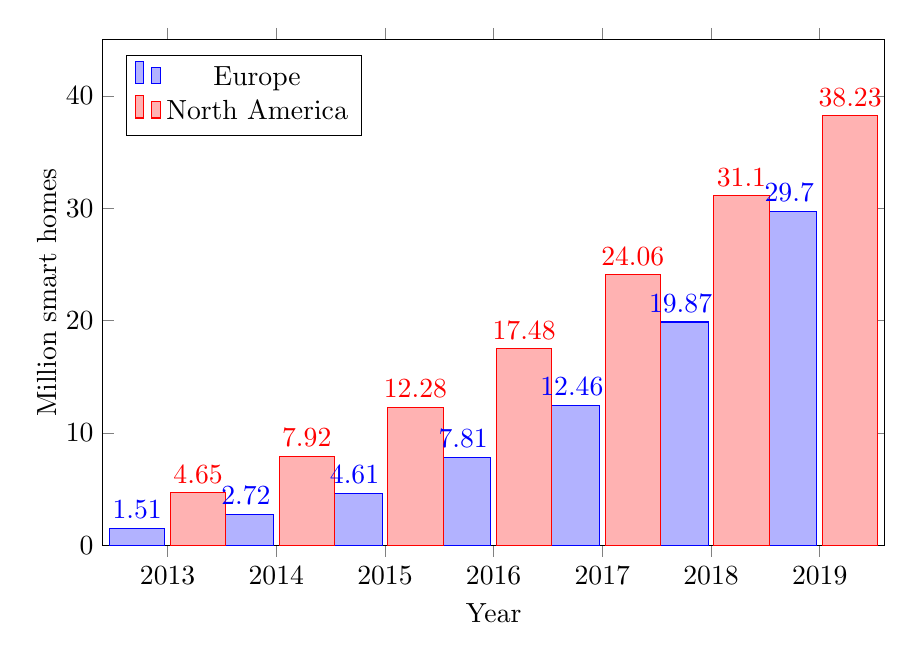
\begin{tikzpicture}
    \begin{axis}[
        height=8cm,
        width=0.95\textwidth,
        xlabel={Year},
        ylabel={Million smart homes},
        yticklabel style={align=right,inner sep=0pt,xshift=-0.3em},
        scaled y ticks = false,
        nodes near coords align={vertical},
        nodes near coords,
        xtick=data,
        symbolic x coords={2013, 2014, 2015, 2016, 2017, 2018, 2019},
        ybar,
        ymax=45,
        ymin=0,
        bar width=20pt,
        legend pos = north west,
        ]
        \addplot coordinates {(2013, 1.51) (2014, 2.72) (2015, 4.61) (2016, 7.81) (2017, 12.46) (2018, 19.87) (2019, 29.70)};        
        \addplot coordinates {(2013, 4.65) (2014, 7.92) (2015, 12.28) (2016, 17.48) (2017, 24.06) (2018, 31.10) (2019, 38.23)};
        \legend{Europe, North America}
        
        %Trend lines:
%        \addplot [ultra thick,orange,line join=round,smooth, nodes near coords = ] coordinates {(2013, 1.51) (2014, 2.72) (2015, 4.61) (2016, 7.81) (2017, 12.46) (2018, 19.87) (2019, 29.70)};
%        \addplot [ultra thick,orange,line join=round,smooth, nodes near coords = ] coordinates {(2013, 4.65) (2014, 7.92) (2015, 12.28) (2016, 17.48) (2017, 24.06) (2018, 31.10) (2019, 38.23)};
%        

    \end{axis}
\end{tikzpicture}
  \caption{Smart homes trend based on sales and statistics. Data from \protect\cite{SMARTHOMETREND}.}
  \label{fig:smarthomestrend}
\end{figure}

The definition of a \emph{smart home system} presented in \cite{SMARTHOMETREND} requires that the system uses a smartphone application or a web portal as a user interface. Therefore the numbers presented in \Cref{fig:smarthomestrend} does not include homes controlled solely by switches, timers, sensors and remote controls and as such the numbers would be higher if the definition was not as strict.

In order for a web portal or a smartphone application to provide meaningful functionality in a smart home system, the software should provide some mechanism for controlling or monitoring devices in the home. In order to do this, the devices are accessible using some technology for exchanging data, \eg~WiFi or Bluetooth. These devices are involved in the concept of Internet of Things. 

While not directly related to the concept of a smart home, a wearable device can play a role in a smart home. The wearable device can provide the application used for interacting with devices in the smart home.

Note that the definition of a smart home as presented in \cite{SMARTHOMETREND} does not include to which degree the smartphone application or web portal is involved in the smart home. A simple system including a smartphone app with a single button for turning a light on and off is regarded a \emph{smart home system}.

We accept the definition of a smart home presented in \cite{SMARTHOMETREND} and formulate it as shown in \Cref{def:smarthome} as it is sufficent for our use in that we are interested in replacing the smartphone app with an app running on wearable device.

\begin{definition}
\label{def:smarthome}
A smart home, is a home that can be controlled using a smartphone application or a web porta as a user interface.
\end{definition}

%%% Local Variables:
%%% mode: latex
%%% TeX-master: "../../master"
%%% End:

\section{Problem Statement}
\label{sec:problem-statement}

It is our hypothesis that we can utilize contextual information to determine which device a user intends to control in a smart home environment. Our problem statement is as follows.

\begin{framed}
\noindent How can we design and implement a system that utilize contextual information for controlling a smart home using a wearable in a gesture driven solution?
\end{framed}

%%% Local Variables:
%%% mode: latex
%%% TeX-master: "../../master"
%%% End:

\section{Target Group}
\label{sec:target-group}

In~\cite[p. 15]{prespecialisation} we defined the target group as people living in a smart home and interested in controlling the state of their home, \eg~lights, music centres, doors and windows, in a convenient matter. The group of people will currently consist of early adoptors of smart home technologies but based on the trend in IoT, our assumption is that the technology will be widespread within 5-10 years. 

We extend the definition of the target group presented in~\cite[p. 15]{prespecialisation} to include a definition of the surroundings. As shown in \Cref{appendix:housing-types:table} the most common size of housings in Denmark is 75-99 square meters. Therefore we assume that the solution presented in this report is installed in a typical Danish apartment with a size of 90 square meters and with 3-4 rooms.

We assume each room has two-three controllable lamps. The living room may have a television and a music centre while the kitchen may have a controllable coffee machine. We estimate that 2-5 controllable devices per room seems fair leaving us with a maximum of 20 controllable devices in an apartment.

%%% Local Variables:
%%% mode: latex
%%% TeX-master: "../../master"
%%% End:

\section{Scenarios}
\label{sec:analysis:scenarios}

\todo[author=Simon]{The requirement specification seem tightly coupled with the scenarios. Does the scenarios belong to the introduction?}

This section describes a few scenarios that might occur during the use of the envisioned system. We make the following assumptions about the system and the environment in which these scenarios take place:

\begin{itemize}
    \item All controllable devices are connected through a central hub.
    \item The system is installed in a private home with clearly defined rooms.
    \item Data about these devices, such as their location and their current state, is always available.
    \item The location of the user is always available when he is in his home.
\end{itemize}

\subsection{Playing Music in the Kitchen}
\label{sec:analysis:scenarios:playing_music}

Assume that a person is in his kitchen and wishes to listen to music while cooking, and that this person has a stereo in the kitchen as well as in the living room that are both connected to his smart hub.
Assume also that this person uses the same set of gestures to control these stereos as they are functionally equivalent and the use of them does not vary enough to warrant separate sets of gestures.
Thus when this person wishes to interact with his stereo by performing the gestures bound to them it is neccesary to determine which stereo is the intended target.

If the gesture performed is set to turn on a stereo, it is relevant to inspect the state of all stereos as it does not make sense to attempt to turn on a stereo that is already turned on.
As well it is relevant to use the location of the person compared to the different steroes, as it is more likely that he intends to control the ones in the same room as him than the ones in other rooms.

Hence if there is a stereo in the kitchen that is not already turned on then it is safe to  assume that that is the intended target of the persons action.

Similarly, if the stereo in the kitchen is already turned on but the one in the living room is not, then the one in the living room is most likely the intended target.

Though not apparent in this example scenario, working with devices such as stereos pose some interesting challenges regarding gesture control as they require more granular control than mere on / off, eg. when controlling the volume at which the music plays.

\subsection{Handling Uncertainties}
\label{sec:analysis:scenarios:handling_uncertainties}

Not all scenarios will work out as well as the one previously presented.
Sometimes a meaningful action cannot be determined from a gesture or the context of the user.
Assume that a person is in his living room and he performs a gesture that is recognized as ``Turn on TV'', but the only TV in the house (located in the living room) is already turned on.
In this case the action could be considered void, but we propose a different solution.
Rather than just ignoring the persons request, a list of alternate actions could be presented to him on his smartwatch.

It may be safe to assume that the person wanted to interact with the TV if the gesture performed was bound to this device, thus the target is still determined from the gesture, the location of the user and the location of the device, just as in the previous scenario.
Which actions would be presented however, could be the inverse of the one performed (if applicable) which in this case would be to turn the TV off.
It could also be a list of the actions most frequently performed by the user.

Another case of uncertainty would be if the gesture performed was not recognized.
This could be considered void and the person would be asked to try again, or the intended target could be assumed to be the device that the person most recently interacted with, and a list of the most frequently used actions could be presented on the persons watch.

\subsection{Controlling Devices in Other Rooms}
\label{sec:analysis:scenarios:other_rooms}

Assume that a person is in his bedroom watching TV but then remembers that he forgot to turn off the TV in the living room.
He wishes to turn off the TV in the living room but not the one located in the bedroom.
If the system follows the logic presented in \cref{sec:analysis:scenarios:playing_music}, then performing a gesture bound to ``Turn off TV'' would turn off the TV in the bedroom as it is in the same room as the person.
To circumvent this, the smartwatch app could allow the user to select which room he would like to control devices in.

%%% Local Variables:
%%% mode: latex
%%% TeX-master: "../../master"
%%% End:

\section{Context}
\label{sec:analysis:context}

In the envisioned system the context is used to determine which actions should be triggered when the user performs a gesture. Therefore the context plays an important part in the envisioned system.

The notion of context is researched in multiple fields, including philosophy and psychology \cite{bolchini2007data}. For the purpose of this project we focus on the notion of context in context-aware software systems. Abowd \etal\cite{abowd1999towards} uses the following definition of the context for context-aware systems:

\begin{italicquote}
Context is any information that can be used to characterize the situation of an entity. An entity is a person, place, or object that is considered relevant to the interaction between a user and an application, including the user and applications themselves.
\end{italicquote}

According to this definition, information is context if the information characterizes the situation of a participant in an interaction \cite{abowd1999towards}.

Consider the following example.

\begin{testexample}
A clothing store has a system installed that sends notifications to users mobile devices with offers when they are near the clothes that the offer apply to. If a t-shirt is 20\% off, and the user is near the t-shirt, the user will receive a notification letting them know that the t-shirt is on sale.
\end{testexample}

In the above example, context includes:

\begin{itemize}
\item The position of the user.
\item The position of the t-shirt on sale.
\item The sex of the user.
\item The age of the user.
\item The percentage the price of the t-shirt is reduced with.
\end{itemize}

Information such as what other customers are in the store and the time of the day is not context because it is not relevant to the interaction between the user and the application.

\subsection{Context Types}

Abowd \etal\cite{abowd1999towards} categorizes context, describing the location, identity, time and activity to be the \emph{primary} context types that answer questions of \emph{where}, \emph{who}, \emph{when} and \emph{what}. Answering these questions help us understand \emph{why} a given situation occurs. In this project an action is triggered on a controllable device because the user is interested in triggering it (that's the \emph{why}).

Abowd \etal~state that \emph{secondary} context types can be derived from the \emph{primary} context types. When the identity of a user is known, additional information can be derived. In the previous example the sex and age of the user are primary context types that can be derived from the identity of the user. 
The price reduction of the t-shirt is secondary information as well as it can be derived from the identity of the t-shirt.
The position of the user and the t-shirt are both primary context types.

\subsection{Context Features}

Abowd \etal\cite{abowd1999towards} defines a context-aware system as follows.

\begin{italicquote}
A system is context-aware if it uses context to provide relevant information and/or services to the user, where relevancy depends on the user's task.
\end{italicquote}

Based on this definition, Ferreira \etal\cite{ferreira2014distributed} outlines the following three main features a context-aware system can provide to its users.

\begin{itemize}
\item Presentation of information and services. Systems with this feature, use context to suggest services to the users or present them with relevant information. Yelp, a service that presents users with nearby businesses, is an example of a system implementing this feature.
\item Automatic execution of a service. Systems with this feature automatically execute a service based on context. Philips Hue, which can automatically change the lighting based on the time of day, is an example of a system implementing this feature.
\item Tagging of context to information for later retrieval. Systems with this feature associate information with context. \cite{ferreira2014distributed} uses a service that tags locations with a virtual note for other users to see as an example of systems implementing this feature.
\end{itemize}

According to the categorization of context-aware systems by Ferreira \etal~the system envisioned in this report belongs to the category of systems implementing automatic execution of a service. Based on context, the system automatically triggers an action on a controllable device. While the user must perform a gesture in order to trigger the action, the system is still automatic as we consider the gesture to be context.

\subsection{Conclusion}

We accept the definitions of context and context-aware systems proposed by Abowd \etal~and the system envisioned in this project makes use of the following context.

\begin{itemize}
\item The position of the user.
\item The gesture performed by the user.
\end{itemize}

Other context can be included in the system but in order to limit the scope of this project, we focus on the position and the gesture.

The system is context-aware as it automatically executes a service when a gesture is performed, provided that an appropriate action to trigger can be determined.

%%% Local Variables:
%%% mode: latex
%%% TeX-master: "../../master"
%%% End:

\section{Controlling a Smart Home}
\label{sec:introduction:gesture-control}
% \todo[author=Kasper]{Vi bør nok lige komme på en bedre titel til dette afsnit.}

Controlling a smart home is a matter of changing the state of smart devices in the home. For example, opening or closing a window, locking or unlocking the door or changing the temperature on the thermostat. There are a variety of ways to control a smart home including, but not limited to, the following.

\begin{itemize}
\item Using a smartphone application.
\item Using a physical remote control such as the Logitech Harmony Remote\footnote{More information about the Logitech Harmony Remote is available at \url{http://www.logitech.com/harmony-remotes}}.
\item Using rules that are automatically triggered when specific events occur, \eg~the time of the day changes.
\end{itemize}

An alternative way of controlling a smart home is using motion gestures using a wearable worn by the user. One survery found that 76\% of 37 people consider gestures a natural way of controlling devices, 8\% found it unnatural and the remaining 16\% left the question unanswered~\cite{Kela2006}.

\subsection{Required Amount of Gestures}

The amount of gestures a person is able to recall is limited. The smaller a set of gestures is, the easier it is for a person to remember. This is supported by~\cite{Kela2006} wherein a user study reported that users would like to be able to use the same gesture for multiple devices and use a small set of gestures.
The ideal size of a gesture set is unknown, in part because people have differing recollection capabilities. Miller~\cite{miller1956magical} theorized that an adult can store $7 \pm 2$ objects in their working memory.
Reuse of gestures across multiple devices results in fewer gestures to remember, but imposes the challenge of making sure that only the user's intended target device reacts to a gesture.

The scenario presented in \Cref{sec:analysis:scenarios} has a total of 30 actions that can be triggered. If we assume there is only one music centre in the apartment that can be controlled from multiple rooms, we can reduce the amount of actions to 24.

If we make a system in which one gesture maps to a single action, a minimum of 24 gestures would be required to control the smart home shown in \Cref{fig:analysis:scenario:apartment}. Previous studies suggests that a user cannot remember 24 gestures and more so, cannot remember which action each of the gestures trigger~\cite{Kela2006,miller1956magical}.

By taking the location of the user into account, we can reduce the number of gestures a user must remember in order to control the smart home.

From the scenario presented in \Cref{sec:analysis:scenarios} it is apparent, that in a gesture controlled system in which the performance of a gesture triggers different actions depending on the room a user is in, the maximum amount of gestures a user must remember equals the number of actions that can be triggered in the room with the most actions.

In the scenario, the living room has a total of eight different actions, making it the room with most actions. Therefore a total of eight different gestures are required in the system.

%%% Local Variables:
%%% mode: latex
%%% TeX-master: "../../master"
%%% End:

\section{Requirements Specification}
\label{sec:requirements-specification}

This section presents the requirements for the solution. The requirements are divided into the following three groupings.

\begin{description}
\item[Functional requirements] These represent the functionality the solution should implement.
\item[Performance requirements] These requirements describe how well the solution should perform in given conditions.
\item[Overall requirements] These are requirements that the system as a whole should fulfill and that does not fit within any of the two other groupings.
\end{description}

\subsection{Functional Requirements}

\begin{description}
\item[Train and recognize gestures] User should be able to train a motion gesture and when trained, the system should be able to recognize the gesture when the user performs the same movement.
\item[Trigger actions on controllable devices using gestures] Users should be able to trigger an action on a controllable device by performing a gesture using a wearable.
\item[Receive feedback if a gesture is not recognized] If a gesture is not recognized, the user should receive feedback. If possible, the system should guess which gestures the user was likely to perform and suggest the actions associated with the guessed gesture to the user.
\item[Context-aware] The system should be context-aware such that different actions may be triggered from the same gesture depending on the other contextual information available. For example, a circular gesture may turn on the TV when the user is in the living room but when the user is in the kitchen, it turns on the lights.
\item[Associate a gesture with actions] The user should be able to associate a gesture with one or more actions that a controllable device can perform. A gesture can only be associated with multiple actions, if the controllable devices to which the action belongs reside in different rooms.
\item[Virtual positioning of users] A user should be able to virtually positioning himself in his home using the wearable. This allows users to perform gestures in one room, while being in another.
\end{description}

\subsection{Performance Requirements}

\begin{description}
\item[Limit the amount of gestures by letting devices share gestures] As described in \Cref{sec:introduction:gesture-control}, users should be able to use the same gestures for multiple devices and thus reduce the overall amount of gestures they need to recall.
\item[Handle 15-20 controllable devices] As described in \Cref{sec:target-group} we assume the system is deployed in an apartment with 3-4 rooms with 2-5 devices in each room. Therefore the system should be able to handle a minimum of 15-20 controllable devices.
\item[Trigger Correct Action] The correct action should be triggered at least 80\% of the time. An action is considered correct if it is the one that the user intended.
\end{description}

\subsection{Overall Requirements}

\begin{description}
\item[Use inexpensive hardware and software] As described in \Cref{sec:target-group} the target group are people living in a smart home, typically in an apartment with a size of 90 square meters. Therefore we are not interested in expensive cooperate solutions when looking at hardware or software.
\item[Not limited to smart devices in line of sight] Reemo, a related solution, limits the user to control devices that are in line of sight. We do not want to have this limitation in our solution.
\end{description}

%%% Local Variables:
%%% mode: latex
%%% TeX-master: "../../master"
%%% End:

\section{Related Work}
\label{sec:related-work}

The following section presents the work of others that relates to the work described in this report as well as the differences between the two.

Various ways of interacting with the systems in a smart home are presented in \cite[pp. 9-10]{cook2007smart} including speech, facial expressions and gestures. The latter of which has been found to be an easy way of interacting with systems \cite[p. 6]{rahman2011motion} and is utilized in the solution presented in this report. In \cite[pp. 2-3]{starner2000gesture} motion gestures are described to be more convenient than regular remotes, as they require the user to be carrying the remote with them or in the case of wall mounted panels, walk up to the remote. Furthermore the paper describes how speech commands may drown in the noise if users are controlling a media center and that interaction using speech is inconvenient in multi-user configurations.

In \cite[pp. 9-11]{prespecialisation} we described Reemo as related work. Reemo is a solution in which users point at devices and control them using motion gestures \cite{reemo:about}. While the company has not released any details about their technology, we can see from their website that the solution is limited to devices within line of sight as receiver must be placed next to each controllable device.

In \cite{caon2011context} a solution for recognizing context-aware motion gestures using multiple Kinects is presented. Users control devices by pointing at them and depending on the current state of the device and the position of the user, different actions are triggered.
The authors use two Kinects to position the user and recognize motion gestures in a living room, requiring a total of 6-8 Kinects in an appartment consisting of 3-4 rooms.

\subsection{Conclusion}

The solution presented in this report differs from the above solutions in the way, that controllable devices are not required to be within line of sight. Users of our solution are able to control all devices within the system froom anywhere in their house.

Furthermore the solution will utilize beacons for positioning users as opposed to Kinects as utilized in \cite{caon2011context}. This lowers entry barrier by decreasing the initial cost as well as the cost for scaling the system to more rooms.

Gestures are used for controlling the smart home as they are convenient and by utilizing the accelerometer, a common component in wearables \cite[pp. 3-4]{prespecialisation}, the user may not need to buy hardware specifically for recognizing gestures is he owns a wearable with an accelerometer and this wearable is supported in the system.


%%% Local Variables:
%%% mode: latex
%%% TeX-master: "../../master"
%%% End:

\section{Overview}
\label{sec:overview}

This section will briefly describe the structure and the content of rest of the report. 


%%% Local Variables:
%%% mode: latex
%%% TeX-master: "../master"
%%% End:


%%%
% BELOW IS THE DEMO CONTENT
%% 

% \section{Introduction}
% % motivation for creating this theme
% \begin{frame}{Introduction}{}
% \begin{block}{Why the AAU Simple beamer theme?}
%   \begin{itemize}
%     \item<1-> During the last couple of years, I have shared the beamer themes named \chref{http://kom.aau.dk/~jkn/latex/latex.php\#beamer_aausidebar}{AAU Sidebar} and \chref{http://kom.aau.dk/~jkn/latex/latex.php\#beamer_aalborg}{Aalborg} on my website \chref{http://kom.aau.dk/~jkn}{http://kom.aau.dk/\textasciitilde jkn}.
%     \item<2-> Both of these themes feature a sidebar in which the table of content and progress are shown.
%     \item<3-> Some people (in particular one - Yes, I am looking at you, Mads) have been asking about an AAU beamer theme without a sidebar. The present theme named \alert{AAU Simple} is precisely that. 
%     \item<4-> Like the \chref{http://kom.aau.dk/~jkn/latex/latex.php\#beamer_aausidebar}{AAU Sidebar} theme, the theme is not really useful to people not affiliated with AAU due to the tight integration between the theme and the round AAU logo. However, everyone is of course encouraged to download and modify the theme according to their own needs. 
%   \end{itemize}
% \end{block}
% \end{frame}
% %%%%%%%%%%%%%%%%

% \subsection{License}
% % the license
% \begin{frame}{Introduction}{License}
%   \begin{itemize}
%     \item<1-> The AAU logo is covered by copyright rules. I have used the logo from \chref{http://aau.designguiden.dk}{http://aau.designguiden.dk}. As long as you use the theme for making presentations in connection with your work at AAU, you are allowed to use the AAU logo.
%     \item<2-> The rest of the theme is provided under the GNU General Public License v. 3 (GPLv3). This basically means that you can redistribute it and/or modify it under the same license. For more information on the GPL license see \chref{http://www.gnu.org/licenses/}{http://www.gnu.org/licenses/}
%   \end{itemize}
% \end{frame}
% %%%%%%%%%%%%%%%%

% \section{Installation}
% % general installation instructions
% \begin{frame}{Installation}
%   The theme consists of four files
%   \begin{enumerate}
%     \item {\tt beamerthemeAAUsimple.sty}
%     \item {\tt beamerinnerthemeAAUsimple.sty}
%     \item {\tt beamerouterthemeAAUsimple.sty}
%     \item {\tt beamercolorthemeAAUsimple.sty}
%   \end{enumerate}
%   The theme can either be installed for local or global use.
%   \pause
%   \begin{block}{Local Installation}
%     The simplest way of installing the theme is by placing the four theme files in the same folder as your presentation. When you download the theme, the four theme files are located in the {\tt local} folder.
%   \end{block}
% \end{frame}

% % general installation instructions
% \begin{frame}{Installation}
%   \begin{block}{Global Installation}
%   \begin{itemize}
%      \item If you wish to make the theme globally available, you must put the files in your local latex directory tree. The location of the root of the local directory tree depends on the operating system and the latex distribution. On the following slides, you can read the instructions for some common setups.
%     \item When you download the theme, the four theme files are embedded in a directory structure (in the {\tt global} folder) ready to be copied directly to the root of your local directory tree.
%     \item On the following slides, we refer to this directory structure as {\tt <dirstruct>}. \alert{Note} that some parts of the directory may already exist if you have installed other packages in your local latex directory tree. If this is the case, you simply merge {\tt <dirstruct>} with your existing setup.
%   \end{itemize}
%   \end{block}
% \end{frame}

% \subsection{GNU/Linux}
% % installation on GNU/Linux
% \begin{frame}{Installation}{GNU/Linux}
%   \begin{block}{Ubuntu with TeX Live}
%     \begin{enumerate}
%       \item Place the {\tt <dirstruct>} in the root of your local latex directory tree. By default it is\\
%         {\tt \textasciitilde /texmf}\\
%         If the root does not exist, create it. The symbol {\tt \textasciitilde} refers to your home folder, i.e., {\tt /home/<username>}
%       \item In a terminal run\\
%         {\tt \$ texhash \textasciitilde /texmf}
%     \end{enumerate}
%   \end{block}
% \end{frame}
% %%%%%%%%%%%%%%%%

% \subsection{Microsoft Windows}
% % installation on Microsoft Windows
% \begin{frame}{Installation}{Microsoft Windows}
%   \begin{block}{Windows with MiKTeX}
%     Apparently, MiKTeX does not include a local latex directory tree by default. Therefore, you first have to create it.
%     \begin{enumerate}
%       \item To do this, create a folder {\tt <somewhere>} named, e.g., {\tt texmf}
%       \item Add this folder in the Roots tab of the MiKTeX Settings dialog
%       \item Place the {\tt <dirstruct>} in your newly created local latex directory tree\\
%     {\tt <somewhere>\textbackslash texmf}\\
%       \item Open the MiKTeX Settings dialog and click Refresh FNDB.
%     \end{enumerate}
%   \end{block}
% \end{frame}
% %%%%%%%%%%%%%%%%

% % installation on Microsoft Windows Cont'd
% \begin{frame}{Installation}{Microsoft Windows}
%   \begin{block}{Windows with TeX Live}
%     In the advanced TeX Live Installer, you can manually change the default position of the root of the local latex directory tree. However, we assume the default position below.
%     \begin{enumerate}
%       \item Place the {\tt <dirstruct>} in your local latex directory tree\\
%         {\tt \%USERPROFILE\%\textbackslash texmf}\\
%         If it does not exist, create it. In XP {\tt \%USERPROFILE\%} is\\
%       {\tt c:\textbackslash Document and Settings\textbackslash<username>}\\
%       by default, and in Vista and above it is by default\\
%       {\tt c:\textbackslash Users\textbackslash<username>}
%       \item Open the TeX Live Manager dialog and select 'Update filename database' under 'Actions'.
%     \end{enumerate}
%   \end{block}
% \end{frame}
% %%%%%%%%%%%%%%%%

% \subsection{Mac OS X}
% % installation on Mac OS X
% \begin{frame}{Installation}{Mac OS X}
%   \begin{block}{Mac OS X with MacTeX}
%      Place the {\tt <dirstruct>} in the root of your local latex directory tree. By default it is\\
%         {\tt \textasciitilde /Library/texmf}\\
%         If the root does not exist, create it. The symbol {\tt \textasciitilde} refers to your home folder, i.e., {\tt /home/<username>}
%   \end{block}
% \end{frame}
% %%%%%%%%%%%%%%%%

% \subsection{Required Packages}
% % list of required packages
% \begin{frame}{Installation}{Required Packages}
%   Of course, you have to have the Beamer class installed. In addition, the theme loads two packages
%   \begin{itemize}
%     \item TikZ\footnote{By the way, TikZ is an awesome package for creating beautiful graphics. If you do not believe me, then have a look at these \chref{http://www.texample.net/tikz/examples/}{online examples} or the \chref{http://tug.ctan.org/tex-archive/graphics/pgf/base/doc/generic/pgf/pgfmanual.pdf}{pgf user manual}. If you want to create beautiful plots, you should use the pgfplots package which is based on TikZ.}
%     \item calc
%   \end{itemize}
%   These packages are very common and should therefore be included in your latex distribution.
% \end{frame}
% %%%%%%%%%%%%%%%%

% \section{User Interface}
% \subsection{Loading the Theme and Theme Options}
% % list of the themes and options
% \begin{frame}{User Interface}{Loading the Theme and Theme Options}
%   \begin{block}{The Presentation Theme}
%     It is very simple to load the presentation theme. Just type\\
%     {\tt \textbackslash usetheme[<options>]\{AAUsimple\}}\\
%     which is exactly the same way other beamer presentation themes are loaded. The presentation theme loads the inner, outer and color AAU Simple theme files and passes the {\tt <options>} on to these files.
%   \end{block}
%   \begin{block}{The Inner Theme}
%     You can load the inner theme directly by\\
%     {\tt \textbackslash useinnertheme\{AAUsimple\}}\\
%     and it has no options.
%   \end{block}
% \end{frame}
% %%%%%%%%%%%%%%%%

% % list of the themes and options
% \begin{frame}{User Interface}{Loading the Theme and Theme Options}
%   \begin{block}{The Outer Theme}
%     You can load the outer theme directly by\\
%     {\tt \textbackslash useoutertheme[<options>]\{AAUsimple\}}\\
%     Currently, the theme options are
%   \begin{itemize}
%     \item {\tt progressstyle=\{fixedCircCnt, movCircCnt, or corner\}}: set how the progress is illustrated. The value {\tt fixedCircCnt} is the default. 
%     \item {\tt rotationcw}: set the direction of the rotation of the progress circle to clockwise instead of counterclockwise. This option has only effect for the circular progress bars.
%     \item {\tt shownavsym}: show the navigation symbols
%   \end{itemize}
%   \end{block}
% \end{frame}
% %%%%%%%%%%%%%%%%

% % list of the themes and options
% \begin{frame}{User Interface}{Loading the Theme and Theme Options}
%   \begin{block}{The Color Theme}
%     You can load the color theme directly by
%     {\tt \textbackslash usecolortheme\{AAUsimple\}}
%   \end{block}
%   \pause
%   \begin{block}{The Color Element {\tt AAUsimple}}
%     The color theme defines a new beamer color element named {\tt AAUsimple} whose foreground and background colors are
%     \begin{itemize}
%       \item fg: {\usebeamercolor[fg]{AAUsimple}light blue (\{RGB\}\{194,193,204\})}
%       \item bg: {\usebeamercolor[bg]{AAUsimple}dark blue (\{RGB\}\{33,26,82\})}
%     \end{itemize}
%     You can use these colors in the standard beamer way by using the command
%     {\tt \textbackslash usebeamercolor[<fg or bg>]\{AAUsimple\}}. See the beamer manual for instructions.\pause Note that this version of the theme is an official AAU version, in accordance with the \chref{http://aau.designguiden.dk/}{AAU design guide}. However, you can easily change it (including the colour of the logo) by following the steps in {\tt beamercolorthemeAAUsimple.sty}.
%   \end{block}
% \end{frame}
% %%%%%%%%%%%%%%%%

% \subsection{Modifying the theme}
% % how to modify the theme
% {\setbeamercolor{AAUsimple}{fg=gray!50,bg=orange!50}
%  \setbeamercolor{structure}{fg=red}
%  \setbeamercolor{frametitle}{use=structure,fg=structure.fg}
%  \setbeamercolor{normal text}{bg=gray!20}
% \begin{frame}{User Interface}{Modifying the Theme}
%   \begin{itemize}
%     \item<1-> The default configuration of fonts, colors, and layout complies with the \chref{http://aau.designguiden.dk}{AAU design guidelines} and is the \alert{official} version of the theme.
%     \item<2-> However, you can modify specific elements of the theme through the templates provided by the beamer class. Please refer to the beamer user manual for instructions.
%     \item<3-> For example, on this slide the following commands have been used
%       \begin{itemize}
%         \item Change the header colours:\\
%         {\tt \textbackslash setbeamercolor\{AAUsimple\}\{fg=blue!20,bg=red!50\}}
%         \item Change the color of the structural elements:\\
%         {\tt \textbackslash setbeamercolor\{structure\}\{fg=black\}}\\
%         \item Change the frame title text color:
%         {\tt \textbackslash setbeamercolor\{frametitle\}\{use=structure, fg=structure.fg\}}
%         \item Change the background color of the text
%         {\tt \textbackslash setbeamercolor\{normal text\}\{bg=gray!20\}}
%       \end{itemize}
%   \end{itemize}
% \end{frame}}
% %%%%%%%%%%%%%%%%

% \subsection{AAU Waves}
% % the AAU Waves background
% \begin{frame}{User Interface}{The AAU Waves Background Image}
% \begin{block}{The AAU Waves Background Image}
% \begin{itemize}
%   \item<1-> In this documentation, the title page frame and the last frame have the AAU waves as the background image. The AAU waves background image can be added to any single frame by wrapping a frame in the following way\\
%   {\tt \{\textbackslash aauwavesbg\\
%     \textbackslash begin\{frame\}[<options>]\{Frame Title\}\{Frame Subtitle\}\\
%     \ldots\\
%     \textbackslash end\{frame\}\}}
%   \item<2-> Ideally, I would like to create a new frame option called {\tt aauwavesbg} which can enable the AAU waves background. However, I have not been able to figure out how such an option can be added. If you know how this can be done, please contact me.
% \end{itemize}
% \end{block}
% \end{frame}
% %%%%%%%%%%%%%%%%

% \subsection{Widescreen Support}
% % Widescreen Support
% \begin{frame}{User Interface}{Widescreen Support}
% \begin{block}{Widescreen Support}
%   Newer projectors and almost any modern TV support a widescreen format such as 16:10 or 16:9. Beamer (>= v. 3.10) supports various aspect ratios of the slides. According to section 8.3 on page 77 of the Beamer user guide v. 3.10, you can write\\
% {\tt\textbackslash documentclass[aspectratio=1610]\{beamer\}}\\
% to get slides with an aspect ratio of 16:10. You can also use 169, 149, 54, 43 (default), and 32 to get other aspect ratios.
% \end{block}
% \end{frame}
% %%%%%%%%%%%%%%%%


% \section{Feedback}
% %\subsection{Known Problems}
% %% known problems
% %\begin{frame}{Feedback}{Known Problems}
% %  \begin{description}
% %    \item[More than 50 slides] Internally, TeX cannot work with numbers exceeding +/-16
% %  \end{description}
% %\end{frame}
% %%%%%%%%%%%%%%%%%

% \subsection{Bugs, Comments and Suggestions}
% % help me iron out the bugs or give me some comment and suggestions
% \begin{frame}{Feedback}{Bugs, Comments and Suggestions}
%   \begin{itemize}
%     \item<1-> There are probably still some bugs in the theme. If you should find one, then please let me know. No bug is too small!
%     \item<2-> Also, please contact me, if you have some exciting new ideas or just some simple usability improvements.
%   \end{itemize}
% \end{frame}
% %%%%%%%%%%%%%%%%

% \subsection{Contact Information}
% % contact information
% \begin{frame}{Feedback}{Contact Information}
% In case you have any comments, suggestions or have found a bug, please do not hesitate to contact me. You can find my contact details below.
%   \begin{center}
%     \insertauthor\\
%     \chref{http://kom.aau.dk/~jkn}{http://kom.aau.dk/\textasciitilde jkn}\\
%     Niels Jernes Vej 12, A6-309\\
%     9220 Aalborg Ø
%   \end{center}
% \end{frame}
% %%%%%%%%%%%%%%%%

% {\aauwavesbg
% \begin{frame}[plain,noframenumbering]
%   \finalpage{Thank you for using this theme!}
% \end{frame}}
% % %%%%%%%%%%%%%%%%

\end{document}

%%% Local Variables:
%%% mode: latex
%%% TeX-master: t
%%% End:
